
% global preamble
\input{preamble}

\begin{document}

\title{South Korea EPU Memo}
\author{Jessica Yu Kyung Koh}
\date{Current version: \today}
\maketitle

\doublespace

\section{Overview}
\label{sec:overview}
The purpose of this memo is to document how we construct South Korea Economic Policy Uncertainty (EPU) Index, which is based on the monthly counts of news articles that are likely to contain information about the economic policy uncertainty in South Korea.\footnote{For more information about the EPU, visit http://www.policyuncertainty.com.} In this document, we present (i) the term set used in our search, (ii) newspapers used, (iii) web-scraping  strategy (iv) methods used in developing the index, (v) results, and (vi) future steps. 

\section{EPU Term Set} 
\label{sec:term}
We select the combination of terms that show the economic policy uncertainty in South Korea. The selected terms are divided into the following three subsets that show uncertainty, economy, and policy, respectively: 
\begin{enumerate}
\item \textbf{Uncertainty-relevant terms:} ``uncertain," ``uncertainty"  
\item \textbf{Economy-relevant terms:} ``economic," ``economy," ``commerce"
\item \textbf{Policy-relevant terms:} ``government," ``Blue House," ``congress," ``authorities," ``legislation," ``tax," ``regulation," ``Bank of Korea," ``central bank," ``deficit," ``WTO," ``law/bill," ``ministry of finance"
\end{enumerate}
Our assumption is that an article containing at least one term from each of the above subsets implies that economic policy uncertainty existed during the time when the article was published. In order to construct the index, we count the number of newspaper articles containing at least one term from each of the above subsets. We perform all searches in Korean, as shown in Table \ref{tab:korean-ver}.

\begin{table}[H] \caption{Term Sets for South Korean EPU Index, with Translations to English} \label{tab:korean-ver}
\centering
\scalebox{0.88}{
\begin{tabular}{| L{2.3cm} | L{4.7cm} | L{4.5cm} | L{5cm} | }
\hline
\textbf{Category} & \textbf{English Terms} & \textbf{Korean Terms} & \textbf{In Korean Characters} \\ 
\hline
U		& uncertainty OR uncertain & bulhwaksilsung OR bulhwaksil & 불확실성 OR 불확실 \\ \hline
E 		& economic OR economy & gyeongje OR gyeongjeui & 경제 OR 경제의 \\
 		& commerce & sangup OR muyeok & 상업 OR 무역 \\ \hline
P		& government & jeongbu & 정부 \\
		& ``Blue House" & Chungwade & 청와대 \\
		& congress		& gukhoe & 국회 \\
		& authorities 	& dangguk & 당국 \\
		& legislation 	& jejeong OR jejeongbu OR ibbub & 제정 OR 제정법 OR 입법 \\
		& tax 			& se		& 세 \\
		& regulation	& gyuje OR tongje OR gyejeong & 규제 OR 통제 OR 규정 \\
		& ``Bank of Korea" & Hankukeunhaeng OR Haneun & 한국은행 OR 한은 \\
		& ``central bank" 		& jungangeunhaeng & 중앙은행 \\
		& deficit			& jukja OR bujok & 적자 OR 부족 \\
		& WTO 				& WTO OR Segye muyeok gigu & WTO OR 세계 무역 기구 \\
		& law/bill			& bub OR buban & 법 OR 법안 \\
		& ``ministry of finance" & gihwaekjaejungbu OR gijaebu & 기획재정부 OR 기재부 \\ \hline
\end{tabular}}
\end{table}

\section{South Korean Newspaper Sources}
\subsection{Major Newspapers}
Table \ref{tab:majornews} shows information on major newspapers in South Korea. If articles of a newspaper are available in multiple sources, we list all of them in the ``Archive" column and show the time period available in each archive. Further information about archives are described in the next section.

For constructing South Korean EPU index, we currently use six newspapers: Donga Ilbo, Kyunghyang, Maeil Economic, Hankyoreh, Hankook Ilbo, and Korea Economic Daily. We do not use Chosun Ilbo and Chungang Ilbo at this stage, as the boolean operators do not function well in the online search engines for those newspapers. Once the websites are fixed, we aim to use articles from these two sources in the future. 


\begin{table}[H]
\caption{Major Newspapers in South Korea} \label{tab:majornews}
\begin{footnotesize}
\begin{tabular}{L{2.6cm} L{2.3cm}  L{2.2cm} L{3.5cm} L{2.1cm} L{2.1cm}}
\toprule
\textbf{Newspaper Name} & \textbf{Political Orientation} & \textbf{Type} & \textbf{Archive} & \textbf{Date Coverage} & \textbf{Boolean Operators} \\ \midrule
Chosun Ilbo & Conservative & Daily News & Chosun Archive & 1920-Present & No \\ \midrule
Chungang Ilbo & Conservative & Daily News & Chungang Website  & 2000-Present & No \\ \midrule
Donga Ilbo & Conservative & Daily News & 1. Donga Archive & 1920-Present & Yes \\
 &  &  & 2. Naver News Library & 1920-1999 & Yes \\ \midrule
Hankook Ilbo & Moderate & Daily News & Big Kinds & 2000-Present & Yes \\ \midrule
Kyunghyang  &  Liberal & Daily News & 1. Naver News Library &  1946-1999 & Yes \\
 &  & & 2. Big Kinds &  1990-Present & Yes \\ \midrule			
Hankyoreh & Liberal & Daily News & 1. Naver News Library & 1988-1999 & Yes \\
 & & & 2. Big Kinds & 1990-Present & Yes \\ \midrule
Maeil Economic & Conservative & Economic & 1. Naver News Library & 1966-1999 & Yes \\
 & & & 2. Big Kinds & 1995-Present & Yes \\ \midrule
Korea Economic & Conservative & Economic & Big Kinds & 1995-Present & Yes \\ \bottomrule
\end{tabular}
\end{footnotesize}
\end{table}


\subsection{Newspaper Search Engines}
Articles from some South Korean newspapers we use are available in comprehensive news archives. There are two major online news archives (Big Kinds and Naver News Library) that collect historical and current articles from various newspaper sources. These archives are the major sources from which we scrape our data, and we utilize these archives as following:
\begin{enumerate}
\item \textbf{Big Kinds:} contains articles that have been published by 36 national and local news sources from 1990 to the current date. We use 5 major newspapers from this archive, which are Kyunghyang News, Maeil Economics, Hankyoreh, Hankook Ilbo, and Korea Economic Daily.
\item \textbf{Naver News Library:} contains news articles from 4 different sources - Donga Ilbo, Kyunghyang News, Maeil Economics, and Hankyoreh - from 1920s to 1999. Since years of the first publication are different for all 4 newspapers, starting dates of the availability of data are also all different. Donga Ilbo goes furtherest back as this newspaper started publishing from April 1920. Other newspapers started publishing in later years. 
\end{enumerate}

Since the post-2000 articles of Donga Ilbo are not available in the above archives, we extract the EPU counts of those articles from Donga Ilbo's own online search engine. Moreover, although the pre-2000 articles of Donga Ilbo are stored in Naver News Library, we use Donga's own archive as it contains more articles over that time period. Except for Donga Ilbo, EPU counts of all other newspapers are web-scraped from either Big Kinds or Naver News Library.

\section{Web-Scraping Strategy}
The first step in constructing the index is to scrape data from news archives. We scrape the monthly counts of EPU articles and the monthly counts of total articles for each newspaper using Perl from search engines mentioned in the previous section. Since the HTML codes that are used to construct the websites are different across websites, we use different Perl scripts to scrape the data from different archives. All the scripts used for web-scraping are stored in the South Korean EPU repository. 

\section{Constructing the Index}
\subsection{Plotting Counts}

Figures \ref{fig:donga} - \ref{fig:koreaecon} show two sets of information: \textbf{(1)} log of monthly total article counts (the left vertical axis) and \textbf{(2)} ratio of monthly raw EPU article counts over monthly total article counts for each newspaper (the right vertical axis). If article counts of a newspaper are extracted from two archive sources, information of both sources are plotted on the same chart. Log of monthly total article counts help us track the months when a newspaper has abnormally low number of articles. 

\subsubsection{Donga Ilbo}

Figure \ref{fig:donga} plots information regarding Donga Ilbo, which goes back furtherest in date among the newspapers we currently use for South Korea. The figure shows some abnormalities regarding the log total counts.

The first two sets of abnormally low total counts are due to forced suspension of publication. From October 1920 to January 1921, Donga Ilbo was forced to stop publishing when it published articles criticizing Japan's forced ruling of Korea. Similarly, Donga Ilbo temporarily suspended publishing from May 1930 and August 1930 due to the censorship. 

The longer period of abnormally low counts of articles is shown in the 1940s. This is because Donga Ilbo discontinued publishing from the period from August 1940 to December 1945 due to the pressures from the Japanese General Government, which continued to colonialize Korea during those periods. 

The figure also shows that the ratio of the EPU articles over total articles significantly differ across archives before the 1980s. This is because the Korean news articles contained a big proportion of Chinese characters in the text. This gradually changed, and articles published after the 1980s mainly contain Korean characters. Naver News Library translates the Chinese characters to Korean characters and allow searches with Korean keywords even for the articles published before the 1980s. However, Donga Archive does not translate Chinese characters, and the search performed in Korean does not capture articles that are mainly written in Chinese characters. This is why the ratio of EPU over total is much higher for Naver News Library than Donga Archive for articles published before the 1980s.  

\begin{landscape}
\begin{figure}[H] \caption{Monthly Information on Raw EPU and Total Counts (Donga Ilbo)} \label{fig:donga}
\begin{center}
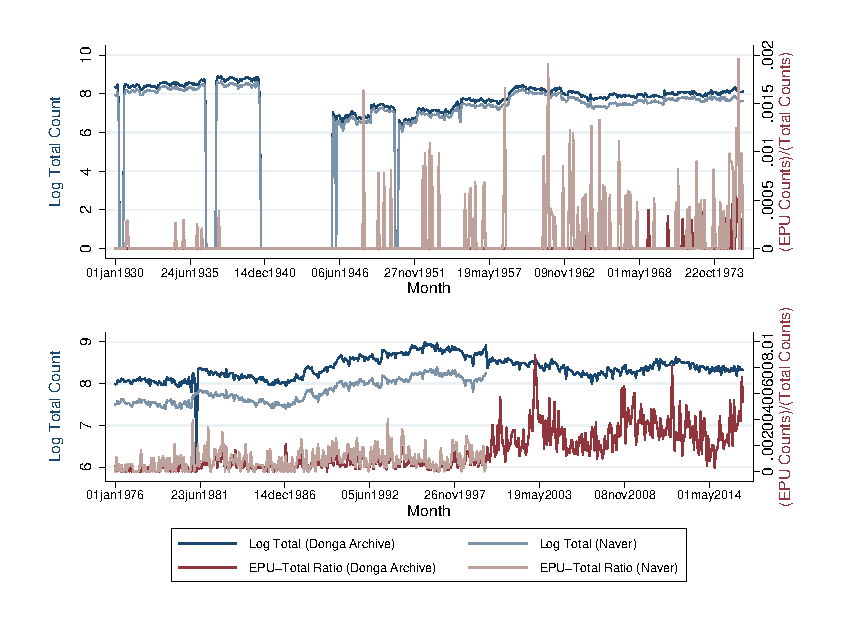
\includegraphics[scale=1.45]{../output/plots/plot_donga_combined.eps} 
\end{center}
\end{figure}
\end{landscape}


\subsubsection{Kyunghyang News}
Figure \ref{fig:kyunghyang} plots information regarding Kyunghyang News, which goes back to 1946. There are a few abnormalities regarding the log total counts of the data before the 1970s due to historical events. 

The first abnormal months is the period between July 1950 and December 1951. According to the written history of Kyunghyang News, there is no evidence that Kyunghyang News discontinued publishing during this period. However, since this period was when the Korean War occurred, it is possible that Kyunghyang News might not have published articles during this period. 

The second abnormal month is December 1952. This is due to the attacks made by the right-wing gang when Kyunghyang News published articles criticizing the the selected amendment bill to the Constitution of South Korea. 

The last set of abonormal months, which is the period between May 1959 to March 1960, occurred because the South Korean government forced Kyunghyang News to stop publishing. This was due to the articles published by Kyunghyang that criticized the fraudulent election that allowed for a prolonged one-man rule by President Seung-man Lee.  

\begin{landscape}
\begin{figure}[H] \caption{Monthly Information on Raw EPU and Total Counts (Kyunghyang)} \label{fig:kyunghyang}
\begin{center}
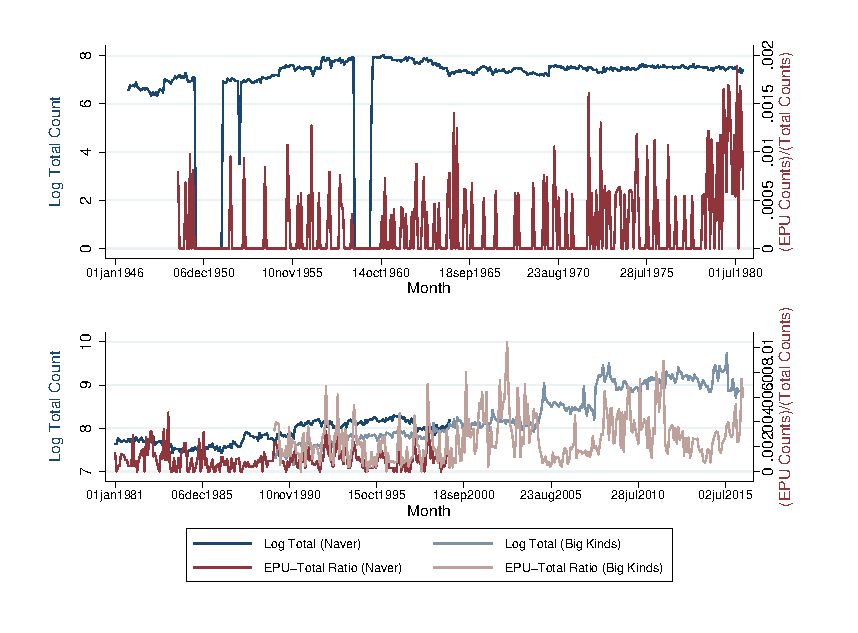
\includegraphics[scale=1.45]{../output/plots/plot_kyunghyang_combined.eps} 
\end{center}		
\end{figure}
\end{landscape}


\subsubsection{Maeil Economic Daily}

Figure \ref{fig:maeil} plots information regarding Maeil Economic Daily, which goes back to 1966. There are no abnormal log counts shown before the 2000s except for the beginning of the publication month. However, there are some abnormally low total counts after the 2000s. However, according to the current evidence, there has not been any suspension of the publication for Maeil Economic Daily after the 2000s. We are currently investigating if this is a problem with the Big Kinds archive. 

\begin{landscape}
\begin{figure}[H] \caption{Monthly Information on Raw EPU and Total Counts (Maeil Economic)} \label{fig:maeil}
\begin{center}
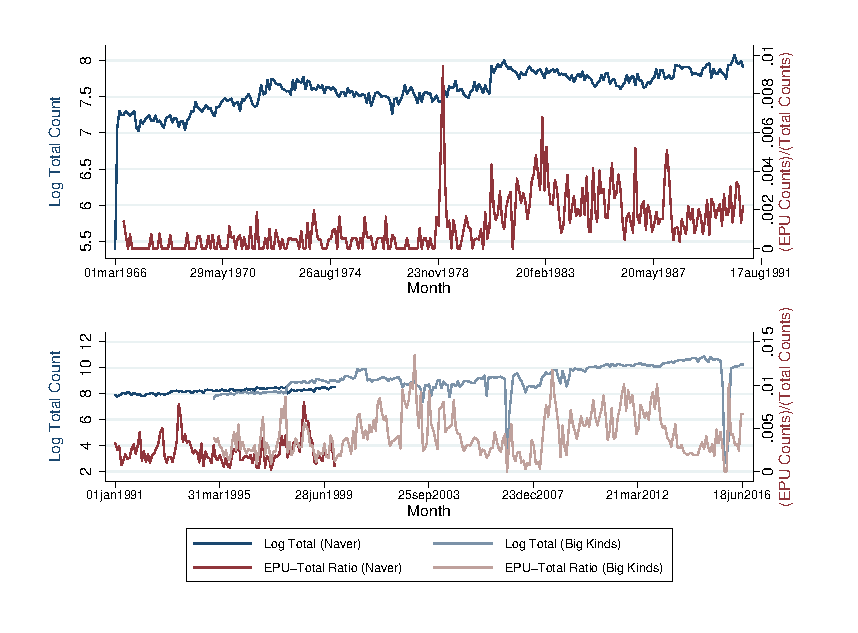
\includegraphics[scale=1.45]{../output/plots/plot_maeil_combined.eps} 
\end{center}
\end{figure}
\end{landscape}


\subsubsection{Hankyoreh}

Figure \ref{fig:hankyoreh} plots information regarding Hankyoreh, which goes back to 1988. According to the figure, there is no noticeable abnormal log total counts for this newspaper. 

\begin{landscape}
\begin{figure}[H] \caption{Monthly Information on Raw EPU and Total Counts (Hankyoreh)} \label{fig:hankyoreh}
\begin{center}
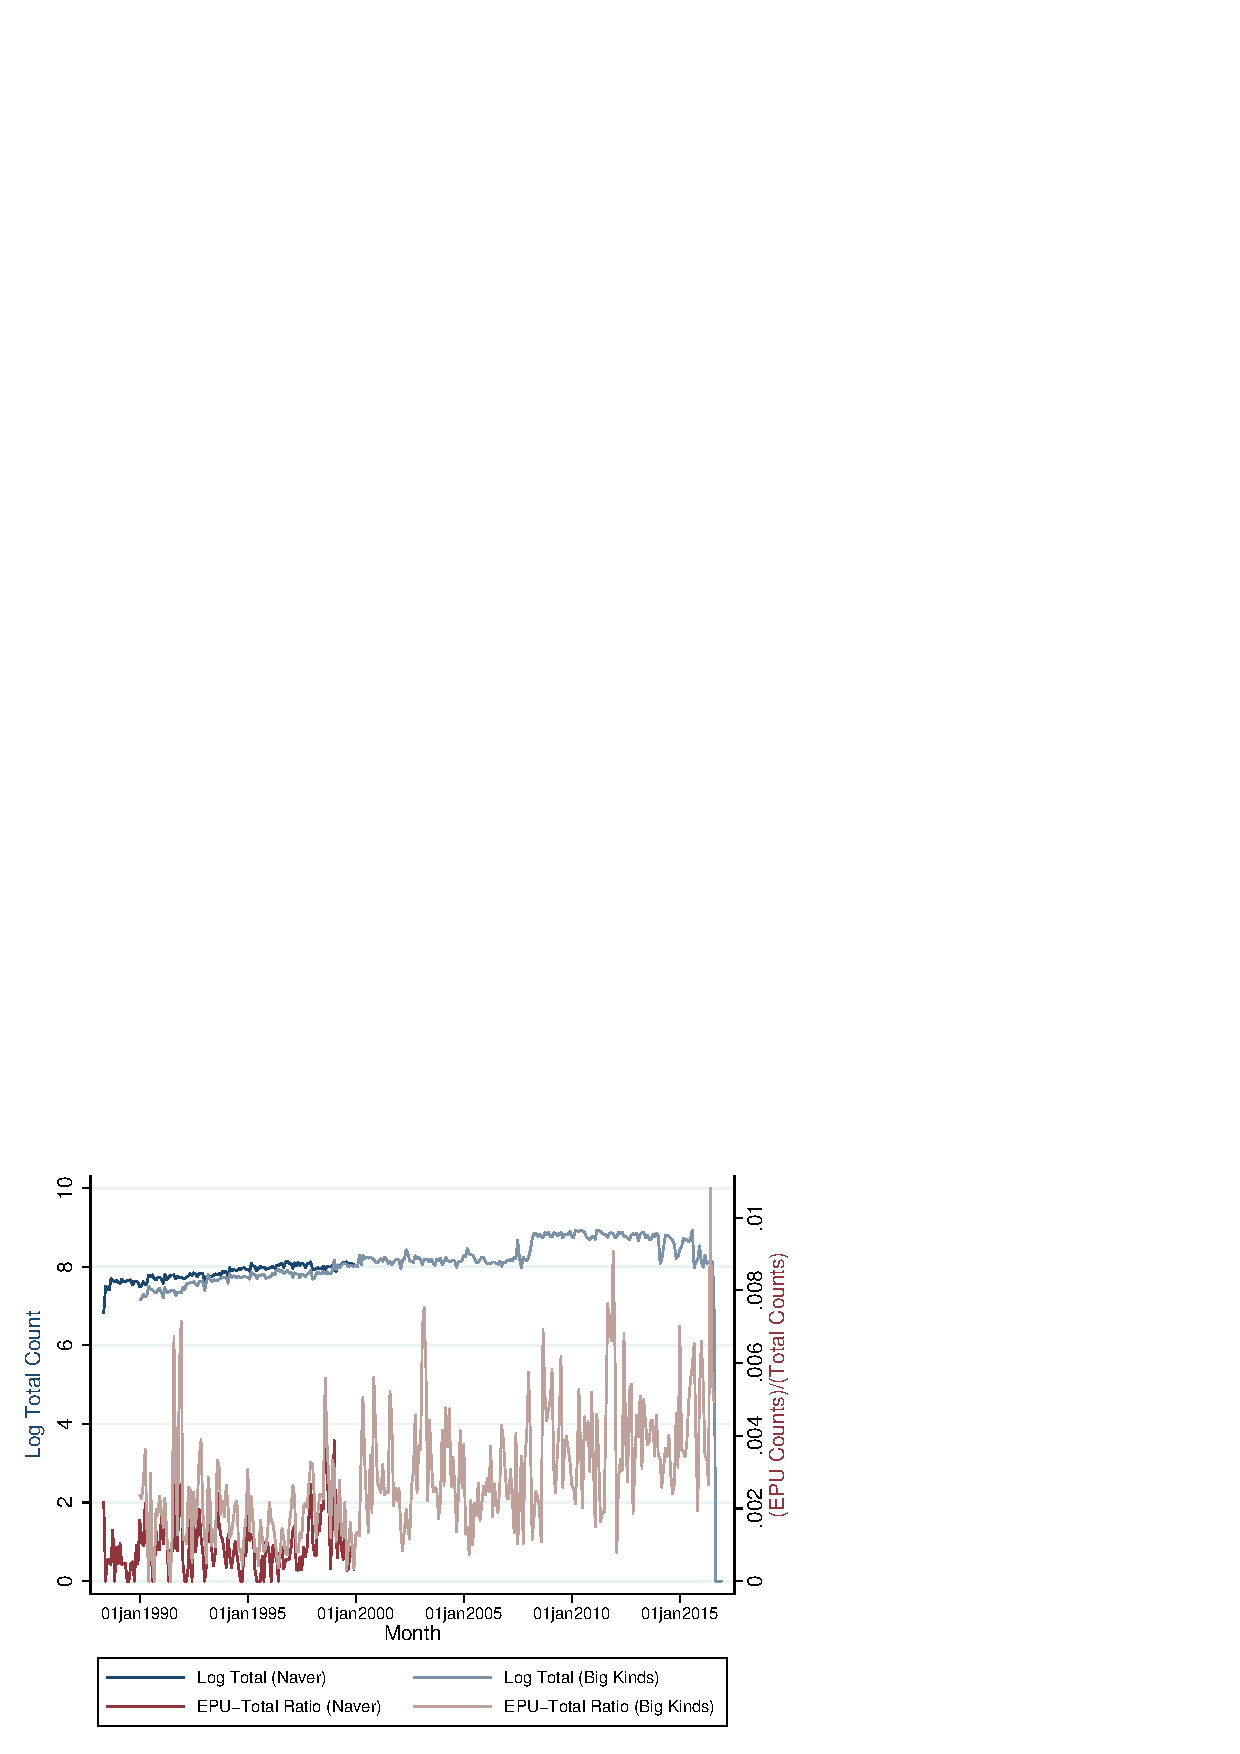
\includegraphics[scale=1.4]{../output/plots/plot_hankyoreh.pdf} 
\end{center}
\end{figure}
\end{landscape}



\subsubsection{Hankook Ilbo}

Figure \ref{fig:hankook} plots information regarding Hankook Ilbo. According to the figure, there is no strong evidence of suspension of the publication for this newspaper. 

\begin{landscape}
\begin{figure}[H] \caption{Monthly Information on Raw EPU and Total Counts (Hankook Ilbo)} \label{fig:hankook}
\begin{center}
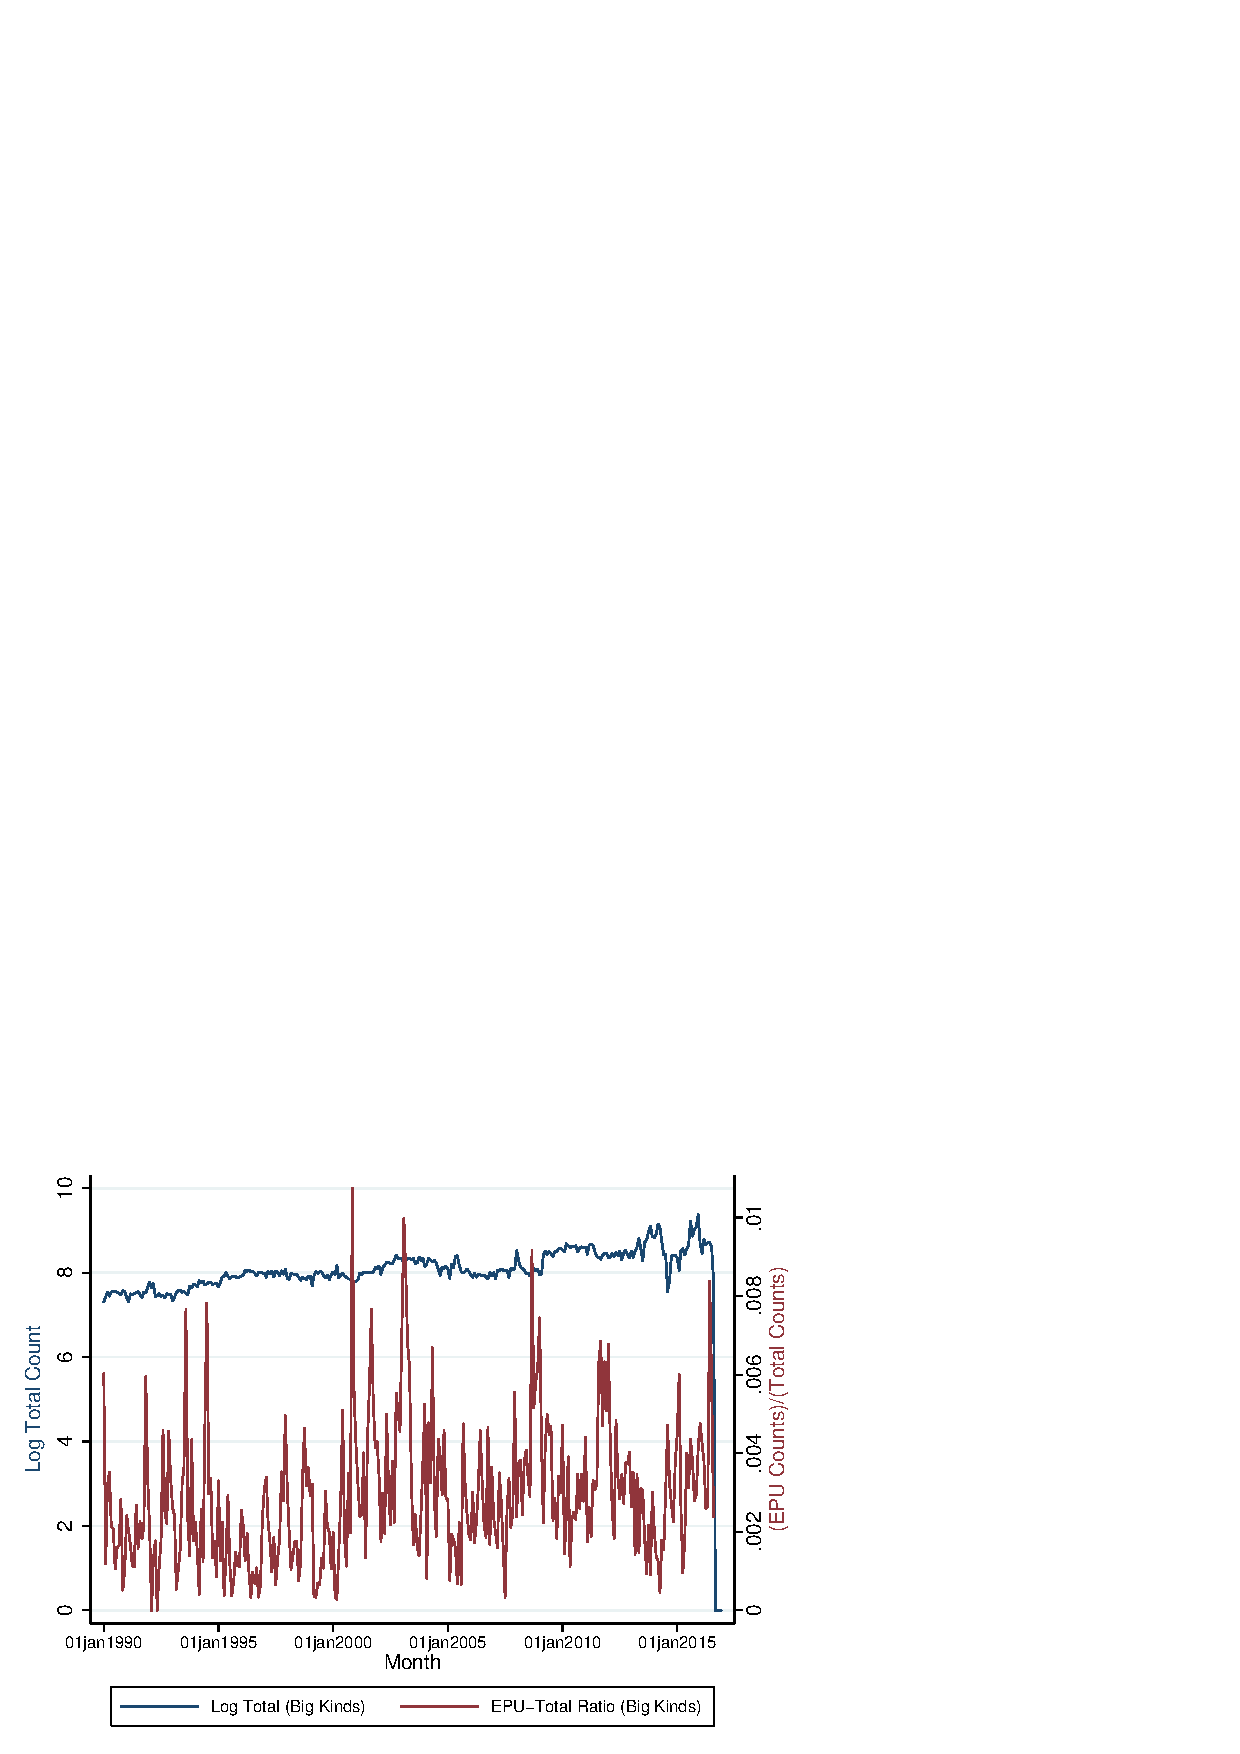
\includegraphics[scale=1.45]{../output/plots/plot_hankook.pdf} 
\end{center}
\end{figure}
\end{landscape}


\subsubsection{Korea Economic Daily}

Figure \ref{fig:koreaecon} plots information regarding Korea Economic Daily. There are some abnormally low total counts shown in the figure. However, according to the current evidence, there has not been any suspension of the publication for Korea Economic Daily during this period. We are currently investigating if this is a problem with the Big Kinds archive. 

\begin{landscape}
\begin{figure}[H] \caption{Monthly Information on Raw EPU and Total Counts (Korea Economic)} \label{fig:koreaecon}
\begin{center}
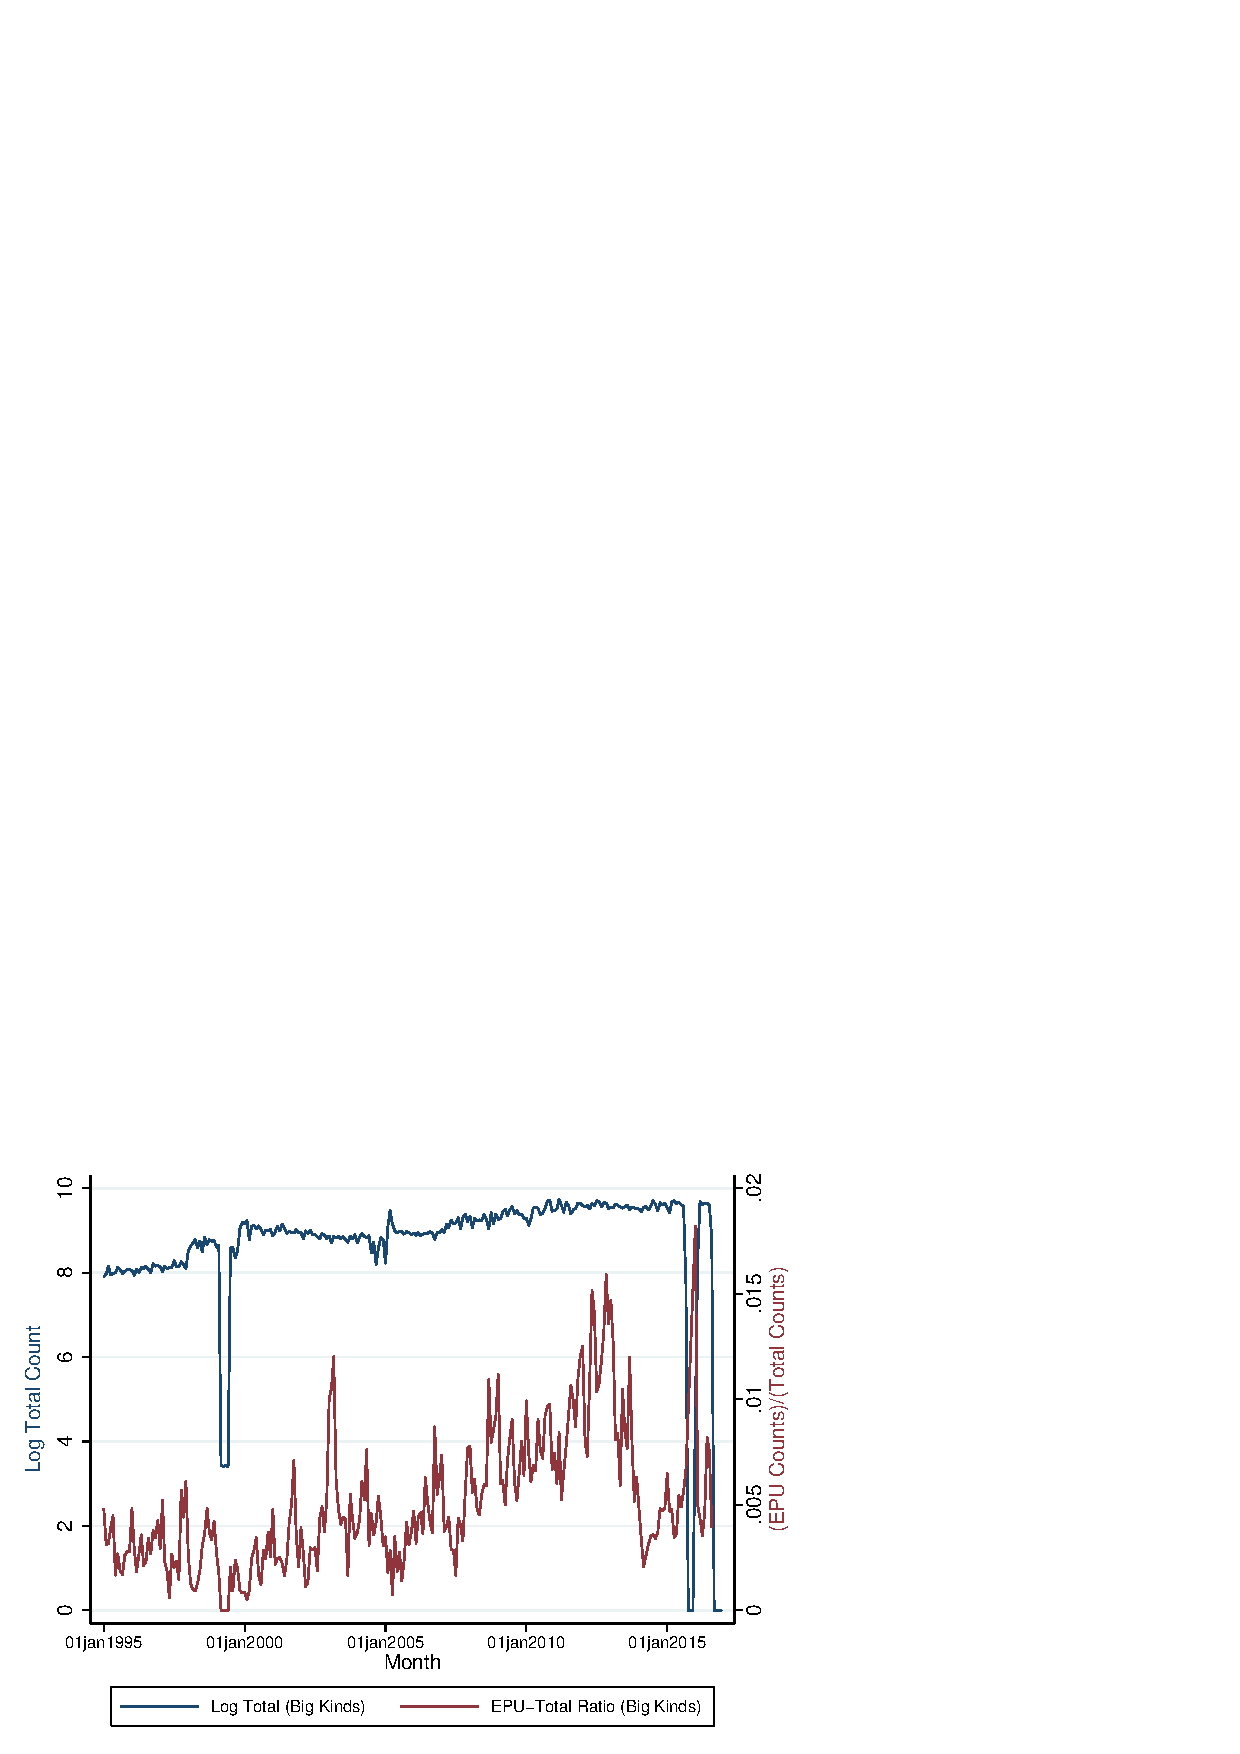
\includegraphics[scale=1.45]{../output/plots/plot_koreaecon.pdf} 
\end{center}
\end{figure}
\end{landscape}

\subsection{Identification of Abnormal Months} \label{subsec:abnormal}

We use the following rule to identify abnormal months for each newspaper in the post-1990 period: Let $N(t)$ be the total newspaper article count in month $t$, and let $\bar{N}(t-15, t-4)$ denote the average monthly article in the same paper from 15 months earlier to 4 months earlier. If $\frac{N(t)}{\bar{N}(t-15,t-4)} < 0.3$, we identify the month $t$ as an ``abnormal month." 

The following list shows abnormal months for each newspaper over the years 1990-2015:
\begin{itemize}
\item \textbf{Hankook Ilbo:} August 2014
\item \textbf{Maeil Economic Daily:} July 2003, December 2006, January - February 2007, September - December 2015
\item \textbf{Korea Economic Daily:} March - June 1999, September - December 2015, January 2016
\end{itemize}

\subsection{Imputation Method}

Each newspaper's raw EPU rate is estimated by dividing monthly EPU article counts over monthly total article counts. However, due to the abnormal months shown in Section \ref{subsec:abnormal}, we use the regression method to deal with the problem and adjust each newspaper's EPU rate for the post-1990 period. 

Let $E^i_t$ be the EPU rate for newspaper $i$ at month $t$. Let $T^{i}$ be the set of abnormal months for newspaper $i$. In order to impute values for the EPU rate during the abnormal months, we first regress EPU rates of a newspaper with abnormal month on EPU rates of newspapers without any abnormal months (which are Donga Ilbo, Kyunghyang, and Hankyoreh). That is,
\begin{equation} \label{eq:imputation}
E^i_t = \alpha + \beta_1 E^{Donga}_t + \beta_2 E^{Kyunghyang}_t + \beta_3 E^{Hankyoreh}_t + \varepsilon^i_t \text{, } \forall t \notin T^i
\end{equation} 

Note that we do not include the abnormal months when estimating the above regression equation. Once Equation \ref{eq:imputation} is estimated, we impute the EPU rates for abnormal months using the following equation:
\begin{equation}
\tilde{E}^i_t = \hat{\alpha} + \hat{\beta_1} E^{Donga}_t + \hat{\beta_2} E^{Kyunghyang}_t + \hat{\beta_3} E^{Hankyoreh}_t \text{, } \forall t \in T^i
\end{equation}

\noindent where $\hat{\alpha}, \hat{\beta_1}, \hat{\beta_2},$ and $\hat{\beta_3}$ are the estimated coefficients from Equation \ref{eq:imputation}. 

\subsection{Standardization Method}

In order to construct an overall South Korean EPU index, we use the adjusted EPU rates that have imputed numbers for abnormal months. We use the following procedures to construct the index:
\begin{enumerate}
\item Multiplicatively standardize each newspaper's adjusted EPU rate so that it has unit standard deviation from January 1995 to December 2014. That is, divide each newspaper's adjusted EPU rate by its raw standard deviation. Our choice of January 1995 as the starting month is because it is the starting month of two of the newspapers used. 
\item Using the normalized EPU rates, average across newspapers by month to obtain an overall South Korean EPU index from January 1990  onward. 
\item Multiplicatively standardize the overall South Korean EPU index to have a mean of 100 from January 1990  to December 2014.
\end{enumerate}

\section{Result}
In this section, we present final outputs of newspaper-level EPU indices and the overall South Korea EPU index. Figure \ref{fig:stdepu_ind}, which is divided into three time periods, shows the standardized newspaper-level EPU indices over time. Figure \ref{fig:stdepu_final} plots the overall South Korean EPU index over time. Since our resources for news articles have changed from last year's South Korea EPU index, we compare the new version of the South Korea index with the old version in Figure \ref{fig:stdepu_final_old}, which shows that there is no noticeable change. 

Figure \ref{fig:annotated} shows the annotated South Korean EPU index over time. Major events that might have contributed to South Korean economic policy uncertainty are marked on the spikes. Those events are selected according to (i) the review of the articles that contains the EPU terms, and (ii) the investigation of the major events occurred during the periods of spikes. 

\begin{landscape}
\begin{figure}[H] \caption{Standardized Newspaper-level EPU Indices} \label{fig:stdepu_ind}
\centering
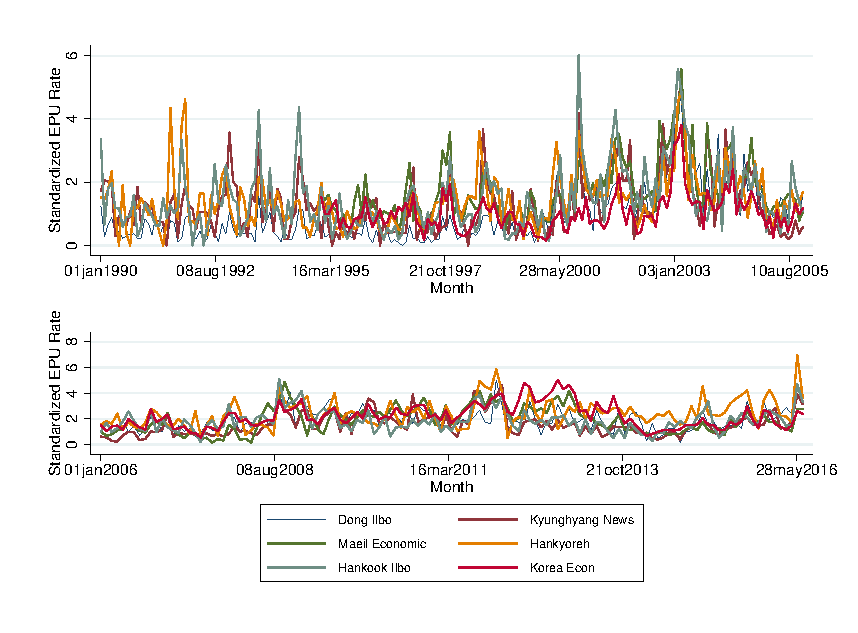
\includegraphics[scale=1.4]{../output/plots/plot_final_combined.eps}	
\end{figure}


\begin{figure}[H] \caption{South Korea EPU Index} \label{fig:stdepu_final}
\centering
		\includegraphics[scale=1.4]{../output/plots/plot_final_skepu.pdf}
		
\end{figure}

\begin{figure}[H] \caption{Comparison of South Korea EPU Index with the 2015 Version} \label{fig:stdepu_final_old}
\centering
		\includegraphics[scale=1.4]{../output/plots/plot_final_skepu_w2015.pdf}
		
\end{figure}

\begin{figure}[H] \caption{Annotated South Korean EPU Index} \label{fig:annotated}
\centering
		\includegraphics[scale=0.85]{../output/plots/annotated-epu-chart.pdf}
		
\end{figure}
\end{landscape}

\section{Next Steps}
\begin{enumerate}
\item Consider furthering the construction of the South Korean EPU index back to the older dates. In order to do so, we need to \textbf{(1)} investigate more into the selection of appropriate terms that capture the economic policy uncertainty and \textbf{(2)} include more newspaper sources, especially Chosun Ilbo, once the archive problems are fixed.
\item Investigate why different news archive show different EPU ratio for same newspaper at some periods. Perform day-level analysis for those periods. 
\item Further document the causes of abnormal months for each newspaper. 
\end{enumerate}

\clearpage


\end{document}